\section{Simulationen}

Die Gleichstrommaschine wird wie in  der Theorie in Simscape modelliert (siehe
Abbildung  \ref{fig:model_dc_motor}).

Die Gleichstrommaschine hat eine maximale Drehzahl von 1000  U/min  bei  einer
maximalen Spannung von \SI{12}{\volt}.

In der elektrischen Dom\"ane befindet sich der Ankerwiderstand  $R_a$  und die
Ankerspule $L_a$. Der elektrische Strom  wird  in  eine  mechanische  Rotation
umgesetzt. Die  Rotation  besitzt  nat\"urlich  ein  Tr\"agheitsmoment  (engl.
\textit{Inertia})  wegen  der  Masse  des  Rotors   und   wird  weiter leicht
ged\"ampft  (engl.   \textit{Rotational   Damper})   weil   der   Rotor  nicht
reibungsfrei ist.

Die physikalischen Gr\"ossen, die f\"ur die Simulation gew\"ahlt wurden, sind:

\begin{threeparttable}
    \centering
    \begin{tabular}{lll}
        \toprule
        Name                   & Zeichen & Gr\"osse \\
        \midrule
        Ankerwiderstand        & $R_a$   & \SI{1}{\ohm} \\
        Ankerinduktivit\"at    & $L_a$   & \SI{0.5}{\henry} \\
        Umsetzungskonstante    & $c\phi$ & \SI{0.1}{\volt\per(\radian\per\second)} \\
        Tr\"agheitsmoment      & $J$     & \SI{0.01}{\kilo\gram\meter\squared} \\
        D\"ampfungsmoment      & $M$     & \SI{0.001}{\newton\meter\per(\radian\per\second)} \\
        \bottomrule
    \end{tabular}
    \caption{}
    \label{tab:dc_motor_values}
\end{threeparttable}

\begin{figure}
    \centering
    \includegraphics[width=.7\linewidth]{images/model_dc_motor}
    \caption{Simscape Modell der Gleichstrommaschine}
    \label{fig:model_dc_motor}
\end{figure}

\begin{figure}
    \centering
    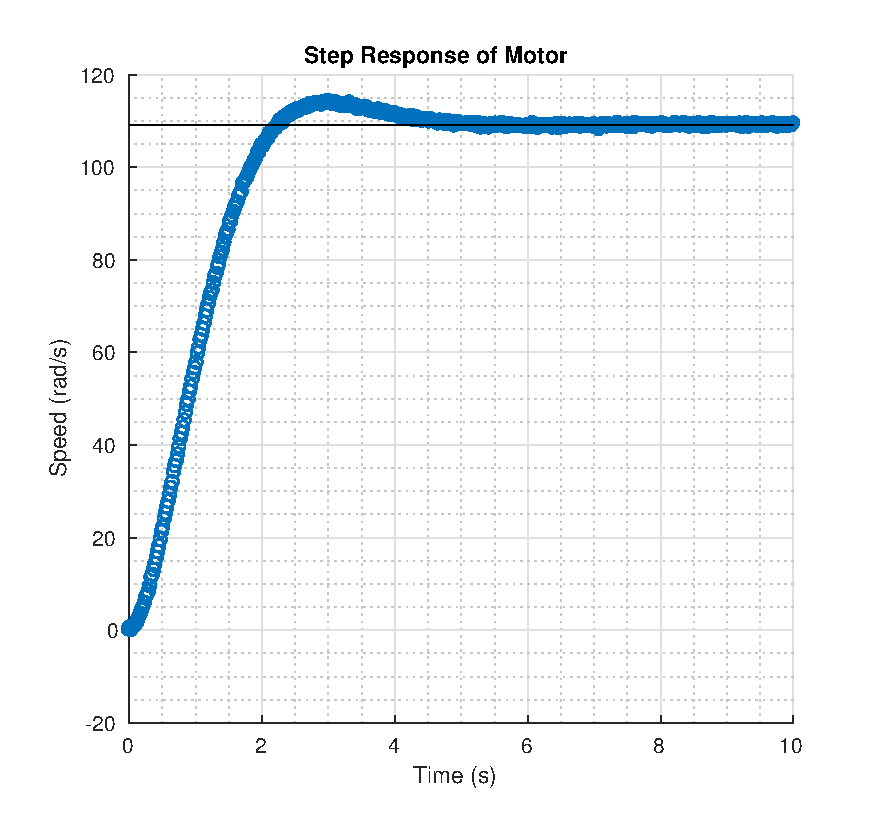
\includegraphics[width=\imagewidth]{images/motor_step}
    \caption{Schrittantwort der Gleichstrommaschine mit \SI{12}{\volt} Eingangsspannung. Die Drehzahl erreicht 1041 U/min, oder \SI{109.1}{\radian\per\second}}
    \label{fig:motor_step}
\end{figure}

Die  Gleichstrommaschine  ist   modelliert.   Eine   erste   Simulation  wurde
durchgef\"uhrt, um die Schrittantwort des Motors zu messen. Diese ist  in  der
Abbildung \ref{fig:motor_step} zu sehen. Wir  sehen,  dass  bei \SI{12}{\volt}
Eingangsspannung      tats\"achlich      die      1000       U/min,       oder
\SI{109.1}{\radian\per\second} erreicht werden.

\begin{figure*}
    \centering
    \includegraphics[width=\imagewidth]{images/model_plant}
    \caption{Simscape Modell der Regelstrecke}
    \label{fig:model_plant}
\end{figure*}

\begin{figure*}
    \centering
    \includegraphics[width=\imagewidth]{images/model}
    \caption{Modell des gesammten Systems.}
    \label{fig:model}
\end{figure*}

\clearpage

Um den Regelkreis implementieren zu k\"onnen m\"ussen die Relevanten Gr\"ossen
gemessen    bzw.    eingestellt    werden   k\"onnen.   In    der    Abbildung
\ref{fig:model_plant} ist dieser Aufbau zu sehen.

Die Speisespannung  des  Motors  wird  mit einer variablen Spannungsquelle von
Simulink  aus  gesteuert.  Die Last am dem Rotor wird auch  von  Simulink  aus
gesteuert.

Die Drehgeschwindigkeit wird  mit  einem  idealen  Drehsensor  gemessen und in
\SI{}{\radian\per\second} an Simulink weitergeleitet.

In   der   Abbildung   \ref{fig:model}   ist   das  Gesamtsystem   zu   sehen.

Um ein bisschen mehr realit\"atsnah zu sein, wird  Rauschen  auf die gemessene
Drehgeschwindigkeit addiert.

Die    gemessene    Drehgeschwindigkeit   wird   zuerst   in    den    Bereich
$[\SI{0}{\volt}..\SI{12}{\volt}$  angepasst, indem die Drehgeschwindigkeit mit
einer  Konstante  von  $0.115$  multipliziert wird. Danach wird sie mit  einer
Periodendauer von \SI{20}{\milli\second} ``abgetastet'' um das Verhalten eines
digitalen  Reglers  zu  simulieren. Die Annahme hier ist, dass der Regler  mit
einem  Mikrocontroller implementiert wird  (sehr  wahrscheinlich  heutzutage).

F\"ur den Regler verwenden wir  den  von  Simulink  zur Verf\"ugung gestellten
\textit{PID Controller} Block.  Davon  gibt  es  eine zeit-kontinuierliche und
zeit-diskrete Version. Wir verwenden die  letztere  und  setzen  auch hier die
Abtastperiode auf \SI{20}{\milli\second}.

L\"asst  man  die Standardeinstellungen  des  PID-Reglers  und  simuliert  das
System, so entsteht --  wie  erwartet  --  nichts  optimales  (siehe Abbildung
\ref{fig:PID_initial}).

\begin{figure}
    \centering
    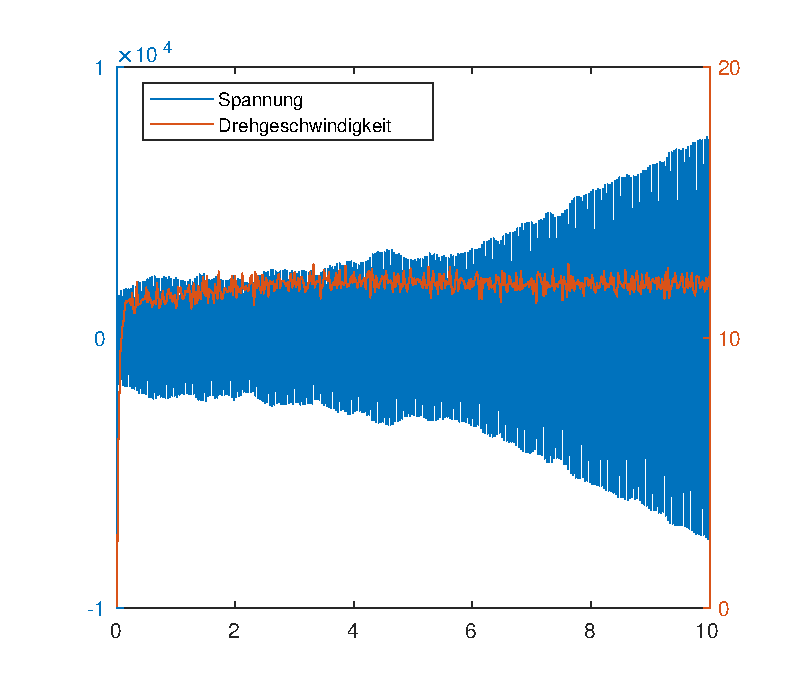
\includegraphics[width=\imagewidth]{images/PID_initial}
    \caption{PID Regler mit Standardeinstellungen. Der Sollwert wird zwar sehr schnell erreicht, aber die Eingangsspannung des Motors schwankt um \SI{10}{\kilo\volt} was f\"ur ein \SI{12}{\volt} Motor nicht optimal ist.}
    \label{fig:PID_initial}
\end{figure}

Die   gr\"osste   Einschr\"ankung   f\"ur   den  Regler   ist   die   maximale
Eingangsspannung des  Motors,  der  zwischen  \SI{0}{\volt} und \SI{12}{\volt}
bleiben muss. Das heisst dass die  Schrittantwort  des  Systems so schnell wie
m\"oglich  sein  sollte,  aber  nicht  so schnell dass diese maximale Spannung
\"uberschritten wird.

Um diese Aufgabe zu l\"osen stellt MATLAB ein PID-Tuning tool zur Verf\"ugung.
Insbesondere  kann  man  die  ``Regleranstrengung''  (engl. \textit{Controller
Effort}) plotten (siehe Abbildung \ref{fig:controller_effort}),  welches sagt,
wie  die  Ausgangsspannung des Reglers verlaufen  wird  wenn  am  Eingang  ein
Schritt von \SI{1}{\volt} angelegt wird.

\begin{figure}[H]
    \centering
    \includegraphics[width=\imagewidth]{images/controller_effort}
    \caption{PID ``Anstrengung'' (engl. \textit{Control Effort}) muss unter den Wert $1.0$ bleiben, damit \SI{12}{\volt} nicht \"uberschritten wird.}
    \label{fig:controller_effort}
\end{figure}

Wenn   die   Reglerkonstanten   also   so   eingestellt   werden,   dass   der
\textit{Controller Effort}  nie  \"uber  den  Wert $1.0$ steigt, dann wird die
Ausgangsspannung    des    Reglers    nie   \"uber   \SI{12}{\volt}   steigen.

